\documentclass[tikz,border=4pt]{standalone}
\usetikzlibrary{arrows.meta,positioning}
\begin{document}
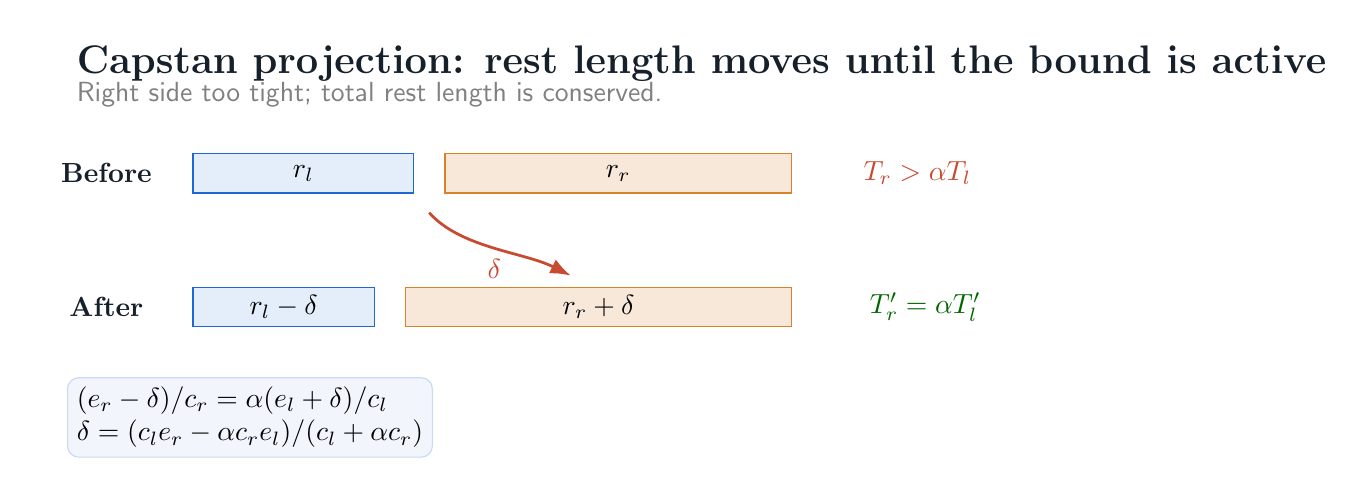
\begin{tikzpicture}[>=Latex, font=\sffamily]
  \definecolor{ink}{HTML}{16202A}
  \definecolor{blue}{HTML}{1F67D2}
  \definecolor{orange}{HTML}{D9822B}
  \definecolor{red}{HTML}{C84B31}
  \draw[fill=white, draw=none] (-0.5,-1.4) rectangle (12.7,4.2);
  \node[anchor=west, font=\bfseries\Large, text=ink] at (0,3.75) {Capstan projection: rest length moves until the bound is active};
  \node[anchor=west, text=gray] at (0,3.35) {Right side too tight; total rest length is conserved.};

  \node[font=\bfseries, text=ink] at (0.5,2.35) {Before};
  \draw[fill=blue!12, draw=blue] (1.6,2.1) rectangle (4.4,2.6);
  \draw[fill=orange!18, draw=orange] (4.8,2.1) rectangle (9.2,2.6);
  \node at (3.0,2.35) {$r_l$};
  \node at (7.0,2.35) {$r_r$};
  \node[red, font=\ttfamily] at (10.8,2.35) {$T_r>\alpha T_l$};

  \draw[->, red, line width=1pt] (4.6,1.85) .. controls (5.0,1.4) and (5.8,1.35) .. (6.4,1.05)
    node[midway, below] {$\delta$};

  \node[font=\bfseries, text=ink] at (0.5,0.65) {After};
  \draw[fill=blue!12, draw=blue] (1.6,0.4) rectangle (3.9,0.9);
  \draw[fill=orange!18, draw=orange] (4.3,0.4) rectangle (9.2,0.9);
  \node at (2.75,0.65) {$r_l-\delta$};
  \node at (6.75,0.65) {$r_r+\delta$};
  \node[green!40!black, font=\ttfamily] at (10.9,0.65) {$T'_r=\alpha T'_l$};

  \node[draw=blue!25, fill=blue!6, rounded corners, anchor=west, align=left, font=\ttfamily] at (0,-0.75)
    {$(e_r-\delta)/c_r=\alpha(e_l+\delta)/c_l$\\$\delta=(c_l e_r-\alpha c_r e_l)/(c_l+\alpha c_r)$};
\end{tikzpicture}
\end{document}
